\documentclass[12pt]{article}
\usepackage[french]{babel}
\usepackage{natbib}
\usepackage{url}
\usepackage[utf8x]{inputenc}
\usepackage{amsmath}
\usepackage{graphicx}
\graphicspath{{images/}}
\usepackage{parskip}
\usepackage{fancyhdr}
\usepackage{vmargin}
\usepackage{listingsutf8}
\lstset{inputencoding=utf8/latin1}

\lstset { %
    language=c++,
    basicstyle=\normalfont\ttfamily,
    numbers=left,
    numberstyle=\scriptsize,
    stepnumber=1,
    numbersep=8pt,
    showstringspaces=false,
    breaklines=true,
    frame=lines,
    backgroundcolor=\color{background},
    literate=
     *{0}{{{\color{numb}0}}}{1}
      {1}{{{\color{numb}1}}}{1}
      {2}{{{\color{numb}2}}}{1}
      {3}{{{\color{numb}3}}}{1}
      {4}{{{\color{numb}4}}}{1}
      {5}{{{\color{numb}5}}}{1}
      {6}{{{\color{numb}6}}}{1}
      {7}{{{\color{numb}7}}}{1}
      {8}{{{\color{numb}8}}}{1}
      {9}{{{\color{numb}9}}}{1}
      {:}{{{\color{punct}{:}}}}{1}
      {,}{{{\color{punct}{,}}}}{1}
      {\{}{{{\color{delim}{\{}}}}{1}
      {\}}{{{\color{delim}{\}}}}}{1}
      {[}{{{\color{delim}{[}}}}{1}
      {]}{{{\color{delim}{]}}}}{1},
}

\usepackage{bera}% optional: just to have a nice mono-spaced font
\usepackage{listings}
\usepackage{xcolor}

\colorlet{punct}{red!60!black}
\definecolor{background}{HTML}{EEEEEE}
\definecolor{delim}{RGB}{20,105,176}
\colorlet{numb}{magenta!60!black}

\lstdefinelanguage{json}{
    basicstyle=\normalfont\ttfamily,
    numbers=left,
    numberstyle=\scriptsize,
    stepnumber=1,
    numbersep=8pt,
    showstringspaces=false,
    breaklines=true,
    frame=lines,
    backgroundcolor=\color{background},
    literate=
     *{0}{{{\color{numb}0}}}{1}
      {1}{{{\color{numb}1}}}{1}
      {2}{{{\color{numb}2}}}{1}
      {3}{{{\color{numb}3}}}{1}
      {4}{{{\color{numb}4}}}{1}
      {5}{{{\color{numb}5}}}{1}
      {6}{{{\color{numb}6}}}{1}
      {7}{{{\color{numb}7}}}{1}
      {8}{{{\color{numb}8}}}{1}
      {9}{{{\color{numb}9}}}{1}
      {:}{{{\color{punct}{:}}}}{1}
      {,}{{{\color{punct}{,}}}}{1}
      {\{}{{{\color{delim}{\{}}}}{1}
      {\}}{{{\color{delim}{\}}}}}{1}
      {[}{{{\color{delim}{[}}}}{1}
      {]}{{{\color{delim}{]}}}}{1},
}


\setmarginsrb{3 cm}{2.5 cm}{3 cm}{2.5 cm}{1 cm}{1.5 cm}{1 cm}{1.5 cm}

\title{Conception architecturale}								% Title
\author{Audrey Eugène \\ Benoit Paquet \\ Michael Faille}								% Author
\date{\today}											% Date

\makeatletter
\let\thetitle\@title
\let\theauthor\@author
\let\thedate\@date
\makeatother

\pagestyle{fancy}
\fancyhf{}
\rhead{\theauthor}
\lhead{\thetitle}
\cfoot{\thepage}

\begin{document}

%%%%%%%%%%%%%%%%%%%%%%%%%%%%%%%%%%%%%%%%%%%%%%%%%%%%%%%%%%%%%%%%%%%%%%%%%%%%%%%%%%%%%%%%%

\begin{titlepage}
	\centering
    \vspace*{0.5 cm}
    
\includegraphics[scale = 0.75]{Logo_UQAM.png}\\[1.0 cm]	% University Logo
    \textsc{\LARGE Université du Québec à Montréal}\\[2.0 cm]	% University Name
	\textsc{\Large MGL7361}\\[0.5 cm]				% Course Code
	\textsc{\large Principes et applications de la conception de logiciels}\\[0.5 cm]				% Course Name
	\rule{\linewidth}{0.2 mm} \\[0.4 cm]
	{ \huge \bfseries \thetitle}\\
	\rule{\linewidth}{0.2 mm} \\[1.5 cm]
	
	\begin{minipage}{0.4\textwidth}
		\begin{flushleft} \large
			\theauthor
			\end{flushleft}
			\end{minipage}~
			\begin{minipage}{0.4\textwidth}
			\begin{flushright} \large
			EUGA21589707 \\
			PAQB01068505 \\
			FAIM02128507 \\
		\end{flushright}
	\end{minipage}\\[2 cm]
	
	{\large \thedate}\\[2 cm]
 
	\vfill
	
\end{titlepage}

%%%%%%%%%%%%%%%%%%%%%%%%%%%%%%%%%%%%%%%%%%%%%%%%%%%%%%%%%%%%%%%%%%%%%%%%%%%%%%%%%%%%%%%%%

\tableofcontents
\pagebreak

%%%%%%%%%%%%%%%%%%%%%%%%%%%%%%%%%%%%%%%%%%%%%%%%%%%%%%%%%%%%%%%%%%%%%%%%%%%%%%%%%%%%%%%%%

\section{Introduction}

Ce travail pratique portera sur le développement d'un jeu vidéo. La conception de ce jeu sera faite dans un langage de programmation fonctionnelle. Nous tenterons donc d'explorer des patrons de conception propres à la programmation fonctionnelle. Ce travail se veut donc exploratoire et expérimental. Comme mentionné à la blague dans la vidéo \cite{functional_video}, les patrons GoF n'ont pas d'équivalents en programmation fonctionnelle. La plupart des patrons pouvant être facilement remplacés par des fonctions. Nous tenterons tout de même d'explorer les meilleures pratiques et notre projet tentera de s'appuyer sur des patrons bien établis dans le milieu autant que possible.

\section{Description du système} 
% : ~ 1 page
% Scope Jeu battleship, expliquer c'est quoi la portée
% Expliquer le concept du jeu (backend seulement)

Le jeu choisi comme base pour l'implémentation est le jeu de société Battleship. Il s'agit d'un jeu qui se joue à deux joueurs. Chaque joueur possède une grille de 11x9 cases qui ressemble à un jeu d'échecs. Sur cette grille, chaque joueur va placer des bateaux de différentes tailles qui occupent un nombre de cases particulier. Par exemple, le porte-avion occupe 5 cases et le torpilleur occupe seulement 2 cases. Chacun des bateaux a une largeur d'une case et les bateaux ne peuvent pas se superposer. La grille des joueurs et le placement des bateaux sont inconnus du joueur adverse. Lorsque les bateaux sont placés, le jeu démarre. Chacun son tour, un joueur va nommer une case. S’il y a un bateau dans cette case dans la grille de l'adversaire, alors le joueur a "touché". Si elle est vide, il a manqué. Les coordonnées nommées par le joueur sont marquées dans la grille de l'adversaire pour qu'il ne demande pas la même coordonnée deux fois. S'il touche toutes les cases d'un bateau, alors celui-ci est coulé. Pour gagner, un joueur doit couler tous les bateaux de son adversaire. Comme les règles sont simples, il est possible d'y jouer avec seulement du papier et des crayons. Il existe aussi un plateau dédié pour y jouer qui est offert en magasin. 

Dans le cadre de ce travail pratique, nous allons faire la conception et l'implémentation du jeu Battleship. Le jeu comportera une architecture client/serveur pour que des joueurs puissent y jouer en ligne. Nous nous concentrerons sur la partie dorsale de l'application. La partie dorsale pourra être découpée en plusieurs services qui pourront faire de l'application des microservices. De plus, nous allons explorer la possibilité d'utiliser le patron architectural "Entity-Component-System", qui est très populaire dans le domaine du jeu vidéo. La partie frontale est hors de la portée du projet. Pour interagir avec le système, il sera possible d'appeler les différents services de l'API exposé par le serveur web.

\section{Description de l’architecture exécutable et des fonctionnalités} 
% : ~ 3-4 pages
% Expliquer le code en détail

\subsection{Analyse}
Dans cette section, nous tenterons d'identifier comment le système sera conceptualisé. La première étape est l'identification des données qui seront utilisées dans le système. Le graphique suivant montre une conception préliminaire des données. Il est possible de voir que le comportement de l'application est restreint à la boîte API et que toutes les données sont dans le reste du graphique. Dans un contexte orienté-objet, la prochaine étape devrait être de transformer nos données dans un ensemble de classes qui interagissent entre elles. Dans notre approche de "AOS vs SOA", qui sera expliquée dans les prochaines sections, nous allons plutôt créer une structure de données complètement indépendante donc découplée du comportement de l'application.

% Pour une raison que j'igonre, ça prend ces tags là
\begin{center}
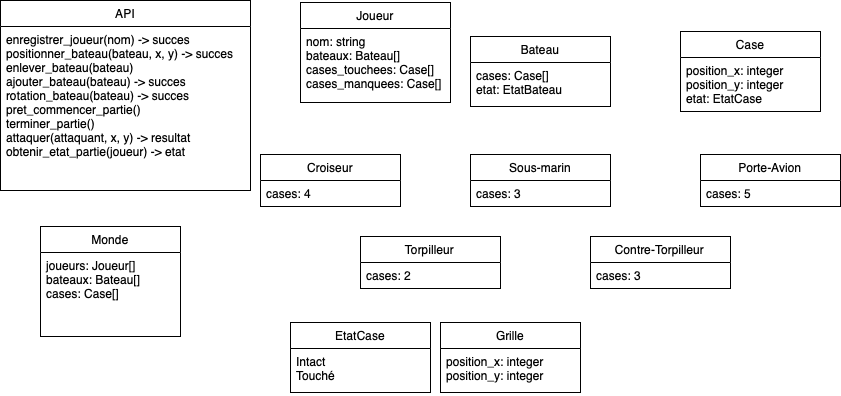
\includegraphics[scale = 0.5]{analyse_tp1.png} \\
Figure: Conception préliminaire de l'application
\\[1.0 cm]
\end{center}

\subsection{Conception}

\subsubsection{Comportement de l'application}

Dans cette section nous présenterons le comportement de l'application. L'objectif est de découpler le comportement de l'application des données ce celle-ci. Pendant la phase d'analyse, les fonctions publiques de l'API ont été identifiées de façon générale. Dans la phase de conception, l'API exposé deviendra plus approfondi et plus détaillé. Dans l'objectif de rester agnostique au langage de programmation dans la phase de conception, la conception de l'API se fera sous forme d'URL dans un fichier bash. Ce genre de fichier peut servir de base pour tester l'application. Le code ci-dessous montre comment appeler les différents services de l'application à l'aide de la commande curl:

\lstinputlisting[language=bash, basicstyle=\tiny]{code/api_call_1.sh}

\subsubsection{Structure de données}

Dans cette section nous présenterons les données de l'application. Ces données seront une structure de données comme il en existe dans les langages de programmation fonctionnels ou qui sont moins stricts sur l'orienté-objet tels le Python ou le JavaScript. Cette structure de données sera présentée au format JSON pour garantir une indépendance du langage de programmation sélectionné. Le code ci-dessous montre un aperçu de la structure de données:

\lstinputlisting[language=json, basicstyle=\small]{code/structure.json}

Cette structure n'est pas complète pour alléger le texte, mais elle contient l'essentiel. À première vue, il peut être difficile quelle est la logique derrière celle-ci. Il est important de rappeler que l'architecture de l'application repose sur les bases de "AOS vs SOA". Comme expliqué dans ce fil de discussion \cite{SOA_AOS_HN}, l'idée est d'organiser les données pour les rendre accessibles avec le même index. Par exemple, le joueur 1 est à l'index 0 et le joueur 2 à l'index 1. Je peux accéder aux données du joueur 1 avec l'index 0 dans la structure de la façon suivante:

\lstinputlisting[language=json, basicstyle=\small]{code/snippet_structure.json}

Cette approche permet d'organiser la mémoire de façon beaucoup plus optimale, en termes d'accès à la mémoire et de cache au niveau du CPU, ce qui peut être très important dans un jeu vidéo. Tel que démontré dans l'article \cite{DOD_Game_Engine}, le moteur de jeu vidéo Ogre 3D l'a appris à ses dépens. En effet, la version 1.0 de celui-ci était largement orientée-objet et à force de grossir en complexité, les performances ont diminué. La version 2.0 a tenté de corriger le tir avec une approche plus centrée sur les données. Bien entendu, comme nous utilisons un langage de programmation qui ne permet pas de contrôler la mémoire, ces avantages seront perdus.

\subsection{Implémentation}

L'implémentation du système n'a pas encore été entamée.

\subsection{Déploiement}

Le graphique suivant montre comment l'application sera exécutée dans un environnement de production. Tout d'abord, l'application sera divisée en deux parties. La première partie contient les services web. La deuxième partie fait la gestion des données de l'application. Comme la partie comportementale et la structure de données ont été bien découplées dès le début, il sera très facile de réorganiser les services à notre guise. Par exemple, il sera possible de déployer l'application en monolithe pour commencer puis de le séparer en plusieurs microservices pour s'adapter à la charge. Il sera aussi possible de dupliquer les services et d'augmenter le nombre de machines. Pour la première itération, tous les services sont déployés sur une seule et même machine virtuelle. Les joueurs s'y connectent à partir de leur propre PC.

\begin{center}
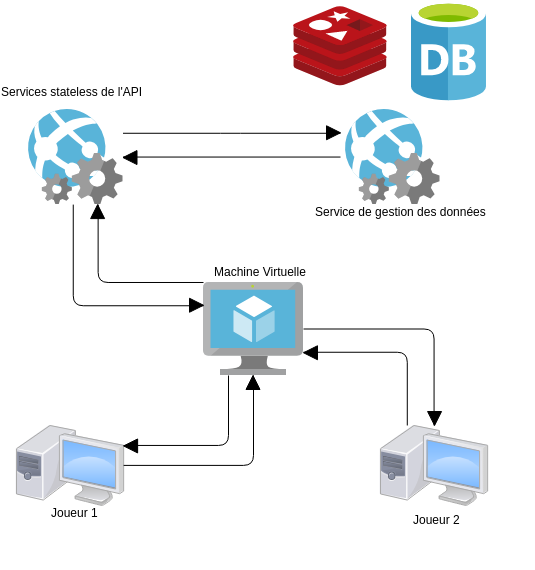
\includegraphics[scale = 0.5]{deploiement.png} \\
Figure: Déploiement de l'application en production
\\[1.0 cm]
\end{center}

\section{Description des styles et patrons architecturaux et/ou de conception} 
% : ~ 2-3 pages
% Expliquer le ECS de façon théorique, plus général
% Expliquer les patrons de conception utilisés de façon théorique
% Architecturaux: ECS, Client/Serveur, Microservices
% Testabilité (fonctions pures)
% ECS + Client/serveur
% Patrons de conception fonctionnels
% https://en.wikipedia.org/wiki/Data-oriented_design
% https://en.wikipedia.org/wiki/Monad_(functional_programming)
% https://news.ycombinator.com/item?id=17977906 (AOS vs SOA)
% https://en.wikipedia.org/wiki/AOS_and_SOA
% Excellent talk sur le functional programming https://www.youtube.com/watch?v=E8I19uA-wGY

\subsection{Styles Architecturaux}

\subsubsection{Style Client/Serveur}

Le style Client/Serveur\cite{client_serveur} consiste en un programme (le client) qui envoie des requêtes à un autre (le serveur) afin d'obtenir des informations ou un service. Ces échanges peuvent se faire par des programmes se trouvant sur un même ordinateur, mais aussi dans le cadre d'un réseau. Dans cette situation, la connexion sera établie via un réseau local (LAN) ou un réseau étendu (WAN). La connexion se termine une fois la requête achevée, c'est-à-dire quand le serveur a retourné les informations ou les services au client. De plus, plusieurs programmes clients peuvent communiquer avec un même programme serveur. Cela a conduit à la création de serveurs spécifiques, qui répondront aux requêtes liées à cette spécification: ils sont appelés daemon. Les points négatifs de ce style sont principalement liés au serveur; en effet, son coût est élevé dû à sa technicité et son importance dans le système fait qu'en cas de panne rien ne va pouvoir se faire. On peut quand même noter que les serveurs sont tolérants aux pannes grâce au système RAID.

\subsubsection{Microservices}

L'architecture Microservices est apparue suite à l'augmentation de logiciels demandant beaucoup de ressources ces dernières années. Ainsi, la solution qu'elle offre pourrait être définie telle qu'expliqué sur le site OpenClassrooms\cite{microservices} : 
\begin{center}
"L'architecture Microservices propose une solution en principe simple : découper une application en petits services, appelés Microservices, parfaitement autonomes qui exposent une API REST que les autres Microservices pourront consommer."
\end{center}
Par conséquent, elle met à disposition des techniques qui aideront à résoudre les difficultés liées aux coûts, à la performance mais aussi à la maintenance. En effet, en séparant les applications en petits services spécifiques, il est plus simple de gérer les mises à jour et les modifications. De plus, en se concentrant sur un aspect spécifique du système la performance devrait s'optimiser tout comme les coûts puisque les idées seront moins dispersées. Chaque microservice communiquera ainsi avec les autres afin de réaliser l'objectif souhaité.

\subsection{Patrons de conception}

\subsubsection{AOS vs SOA}

"AOS and SOA" sont des abréviations anglaises voulant dire "Array of Structures" et "Structure of Arrays" respectivement. Il s'agit de la façon dont les données sont organisées dans une application. Array of Structures désignant une façon d'organiser les données autour des structures. Par exemple, dans un jeu vidéo il pourrait y avoir un objet "World" qui contient une liste d'objets "Player". Ces objets contiennent des attributs propres aux différents joueurs. Cette approche est particulièrement commune dans les jeux vidéos qui sont écrits dans un langage de programmation orientée objet. L'approche "Structure of Arrays" tente l'approche inversée. Au lieu de créer une hiérarchie d'objets, il existe une structure de base qui contient des listes des attributs. Par exemple, il pourrait encore y avoir un objet "World" mais au lieu d'avoir une liste d'objets "Player", les attributs des joueurs sont stockés directement dans des listes de l'objet World. Le code suivant provenant de la discussion \cite{SOA_AOS_HN} donne un excellent exemple de l'inversion de la structure:

\lstinputlisting[language=c++, basicstyle=\small]{code/AOS_SOA.cpp}

\subsubsection{Data-Oriented-Design}

L'approche "Data-Oriented-Design" met l'emphase sur les données d'abord et avant tout. Contrairement à la programmation orientée-objet, où les données et les fonctionnalités sont regroupées sous le concept des classes et des objets. L'avantage de cette approche est qu'elle facilite grandement la compréhension des choses pour le programmeur. En effet, il est beaucoup plus facile d'observer un objet dans la vraie vie et de penser à ses fonctionnalités et ses attributs que de les voir comment étant deux choses distinctes. Cela dit, cette approche n'est pas sans conséquence. Par exemple, le couplage des fonctionnalités avec les données rend la réutilisation de la fonctionnalité beaucoup plus difficile.  Un autre désavantage de la programmation orientée-objet est la gestion moins efficace de la mémoire. En effet, tel que démontré dans l'article "Data-Oriented vs Object-Oriented Design" \cite{data_oriented_design}, l'organisation de la mémoire lorsque les données sont séparées en objets se fait de la façon suivante:

\begin{center}
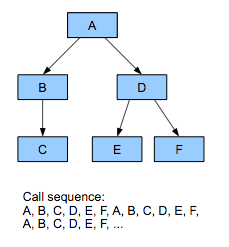
\includegraphics[scale = 0.75]{1_qfwHVxcEq7XQjASYCClQpg.png} \\
Exemple d'appels d'objets pour accéder à la mémoire.\cite{data_oriented_design}
\\[1.0 cm]
\end{center}

Dans une approche orientée données, les données sont plutôt organisées de cette façon:

\begin{center}
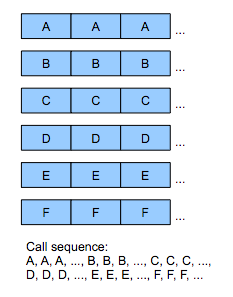
\includegraphics[scale = 0.75]{1_T4XqlgosIzMA_WLzlKWyEw.png} \\
Exemple de l'utilisation de la mémoire en DOD.\cite{data_oriented_design}
\\[1.0 cm]
\end{center}

Dans cette approche, les données similaires sont regroupées ensemble dans un même espace mémoire. Cela a comme conséquence de faciliter l'accès à celle-ci et de faire une meilleure usage du cache du CPU. Il est aussi plus facile de paralléliser le traitement puisqu'il est possible de mieux cibler quelles fonctions utilisent quelle partie de la mémoire. Dans le contexte de notre projet, il pourrait être possible de séparer les données sur plusieurs services spécialisés. Par exemple, un seul service serait responsable de gérer les torpilleurs et un autre service s'occuperait des porte-avions, etc.

\subsubsection{Composition}

La composition est un concept de la programmation fonctionnelle. Elle consiste à considérer les fonctions comme des blocs Lego qui s'empilent et s'emboîtent les unes dans les autres pour créer des couches d'abstractions. Cette façon de penser se rapproche du design atomique \cite{Atomic_Design} qui est une façon populaire de créer des interfaces graphiques de façon méthodique. La composition est très bien expliquée dans la vidéo de Scott Wlaschin \cite{functional_video}. Dans la vidéo la composition est présentée de la façon suivante. On commence par créer des fonctions de bas niveau. Par exemple, une fonction pour mettre les lettres dans une string en majuscule. Ensuite, on prend ces fonctions de bas niveau pour créer des services, par exemple un service pour valider des adresses. On prend ces services et on les combine pour former des use cases. Un exemple de use-case pourrait être de mettre à jour l'adresse. Finalement on combine les use-cases pour former une application web. Évidemment il s'agit d'un exemple parmi tant d'autres pour former composer une application en fonctions de façon structurée.

\section{Description des choix technologiques} 
% : ~ 2 pages
% Expliquer Elixir
% Expliquer Phoenix
% Expliquer les autres technos
% Expliquer pourquoi

Pour développer notre système, nous avons pensé à faire usage de technologies telles que le langage fonctionnel Elixir, le framwork web Phoenix et MongoDB. Nous allons également utiliser des outils tels que des containers pour la réalisation du Battleship.

Intéressons-nous tout d'abord à Elixir\cite{elixir_doc}: il s'agit d'un langage de programmation fonctionnel qui se repose sur la machine virtuelle Erlang (BEAM). Cette dernière étant un ancien système, développé par un système de téléphonie, conçu pour l'exécution de systèmes distribués tout en étant un système "fault tolerant". Cela lui permet une forte disponibilité (avec très peu de plantage) et d'avoir la possibilité de faire des mises à jour sans avoir à relancer le système (rechargement à chaud). Il est également utile dans les domaines de développement web et du logiciel embarqué.
Étant un langage fonctionnel, Elixir va vouloir privilégier du code court, rapide, mais aussi maintenable\cite{elixir_video}. De ce fait, Elixir s'opère à travers des processus isolés qui s'échangent les informations par messages. Ces processus s'exécutent simultanément en grand nombre sur un même ordinateur et peuvent communiquer avec les processus d'autres machines du même réseau. Cela facilite la distribution et la coordination du travail par les développeurs. De plus, l'utilisation de l'isolation permet de collecter ces processus de façon indépendante tout en diminuant les pauses qui se font au niveau du système. Elle fait également en sorte de se servir de toutes les ressources de la machine aussi efficacement que possible: ce que l'on appelle la mise à l'échelle verticale.
En bénéficiant de l'aspect "fault tolerant" d'Erlang, il procure la méthode à suivre pour revenir à un système originel dont la fonctionnalité est garantie lorsqu'une panne aura lieu. Cette caractéristique nous assure d'avoir un système "fonctionnel" en "permanence", le temps que le problème soit corrigé sans que cela affecte les autres réseaux. 

En ce qui concerne la mise en place de notre Battleship, nous avons décidé d'avoir recourt à Phoenix\cite{phoenix} qui est un framework de développement web écrit en Elixir implémentant le modèle MVC côté serveur. Il possède de nombreuses fonctionnalités intéressantes pour notre projet ainsi que des performances applicatives élevées. Il s'avèrera donc particulièrement utile et pratique à notre travail puisque nous pourrons travailler efficacement tout en comprenant correctement le système que nous mettons en place.

Au travers de cet exercice, nous voulions également accroître nos connaissances et nos capacités de programmation avec une technologie nouvelle. Cependant, il fallait s'assurer que cela demeurerait réalisable dans le cadre du projet. C'est pour cela que nous avons décidé de nous servir d'Elixir: c'est un langage intéressant avec une certaine complexité pour notre projet. En effet, nous avons vu que son utilisation pour la programmation de jeux est plus compliquée que les autres, mais reste réalisable sans trop de difficultés.
Ainsi, Phoenix nous a paru comme le meilleur moyen de mettre en place notre Battleship en Elixir.
Pour notre projet, nous avons imaginé un déploiement en microservices avec l'état de l'application dans MongoDB qui est une base de données NoSQL orienté document contenant ses données en JSON. En effet, le state de notre application en JSON s'accorde parfaitement avec MongoDB et présente correctement les éléments que nous avons définis dans notre architecture. Les containers ont été pensés pour l'exécution de services que nous allons mettre en oeuvre avec Elixir.

\section{Conclusion}

En définitive, nous vous avons présenté le Batlleship que nous souhaitons réaliser pour ce projet ainsi que son architecture. Ce travail nous a permis de faire des recherches plus approfondies sur le système que nous mettons en place. De ce fait, nous avons pu présenter et faire usage des patrons précédents qui sont bien établis dans le milieu et propices à ce que nous voulons développer. La réalisation de notre jeu vidéo s'est donc entamée sur des bases solides et claires pour garantir une fonctionnalité favorable par la suite.

\newpage
\bibliographystyle{plain}
\bibliography{biblist}

\end{document}